\subsubsection{Internal Interfaces}
\paragraph{Interface between Accounting and Authentication System}
The interface provided by Accounting component is used by the Authentication System to verify the provided staffID and password.
\subparagraph{Design Rationale:}
\begin{itemize}
	\item Authentication System sends the given staffID and password parameters to the Accounting component.
	\item Based on the type of the staff Accounting checks the password using checkPassword operation belongs to either Admins or Maintainers parts.
	\item Returns the result of the checkPassword operation.
\end{itemize}
\paragraph{Interface between Authentication System and Report Handler}
The interface provided by the Report Handler is used by the Authentication System to report suspicious and wrong login attempts.
\subparagraph{Design Rationale:}
\begin{itemize}
	\item If the boolean result returned by the Accounting, Authentication System sends the provided information to the Report Handler.
	\item Report Handler saves the Login Attempt Log created by the Login Log Writer part in the loginLogs list. 
\end{itemize}
\paragraph{Interface between Accounting and Report Handler}
The interface provided by the Report Handler is used by the Accounting and especially its subcomponent Maintainers to display and check the written System Logs.
\subparagraph{Design Rationale:}
\begin{itemize}
	\item Report Handler provides the loginLogs list and hardwareLogs list to the Accounting and specifically Maintainers part to allow maintainers to use View System Logs function.
\end{itemize}
\paragraph{Interface between Report Handler and Display Controller and Position Controller}
The interface provided by the Report Handler is used by both Display and Position Controllers to report any hardware related technical issues.
\subparagraph{Design Rationale:}
\begin{itemize}
	\item Since Display and Position Controllers are related to hardware devices (camera and motors), it is possible to have hardware related issues. This interface is for handling the hardware related problems.
	\item Report Handler saves the Failure Log created by the Hardware Log Writer part in the hardwareLogs list. 
\end{itemize}
\paragraph{Interface between Display Controller and Position Controller}
The interface provided by the Position Controller is used by the Display Controller for the scanArea operation. In this operation by using this interface Display Controller is able to iteratively move the camera position to scan the area.
\subparagraph{Design Rationale:}
\begin{itemize}
	\item To be able to use Scan function defined in the use-case diagram Display Controller serves scanArea function.
	\item To use the scanArea function position of the stage should be shifted iteratively. Position Controller serves this interface to allow Display Controller to shift stage position in each iteration.
\end{itemize}
\paragraph{Interface between Display Controller and Gallery}
The interface provided by the Gallery is used by the Display Controller to save the captured Images, scans, recorded videos.
\subparagraph{Design Rationale:}
\begin{itemize}
	\item Display Controller is responsible to implement Capture Image, Record Video and Scan functions defined in use-case diagram.
	\item To be able to store the media generated by the Display Controller, Gallery serves this interface.
\end{itemize}
\subsubsection{External Interfaces}
	\paragraph{User Interfaces}
	\begin{itemize}
		\item \textbf{User Web Interface} \\
		Users use a web interface written in javascript using Vue.js framework which is running inside the local microscope server. User can reach to  the User Web Interface by just typing the ip address and designated port of the microscope's server in their browser. Users are able to control the microscope and view the camera feed using the user interface. User Web Interface provides live stream camera feed, navigation menu to change the position of the stage and gallery to view and update the saved media. \\
		\textbf{Design Rationale:} 
		\begin{enumerate}
			\item User web interface has a very simple design to allow inexperienced users to use the provided features easily.
			\item It has a help window that contains solutions for the frequently faced problems to guide users faced with such problems.
			\item The icons have been placed inside the tab buttons in addition to button labels to ensure that the desired feature can be found easily.
		\end{enumerate}
		\begin{figure}[H]
			\centering
			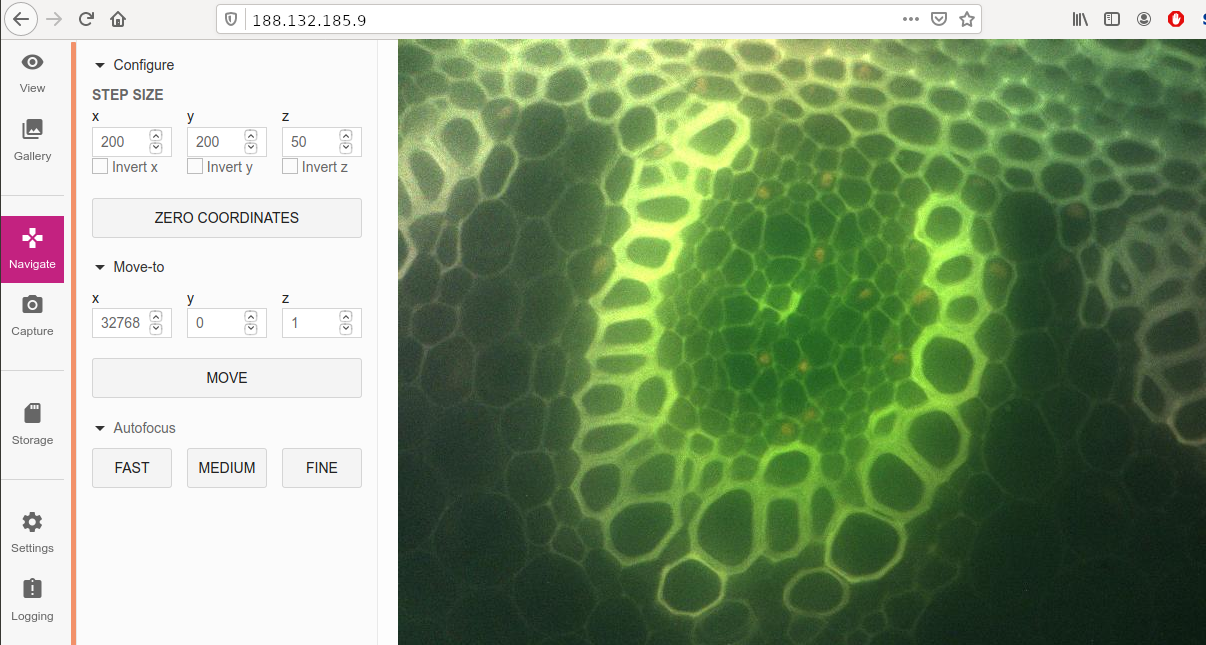
\includegraphics[scale=0.3]{Figures/user_web_interface}
			\caption{OpenFlexure User Web Interface}
			\label{fig:user_web_interface}
		\end{figure}
		\item \textbf{Admin Command-line Interface} \\
		System administrators use a command-line interface to manage the system. Administrators are able to list the detailed information about connected/blocked users such as User IPs, block/unblock status, and connection time. Using the commands provided by this interface, the administrators can view/manage/update system settings and block/unblock users. Admin command-line interface is provided by a bash script placed inside the local microscope server and starts to run when an admin connects to the microscope using SSH. \\
		\textbf{Design Rationale:} 
		\begin{enumerate}
			\item The reason to use a command-line interface rather than GUI is related to speed. Administrators should be able to apply their actions immediately. Since the command-line interface is a more quick way to apply actions, it is preferred over GUI.
		\end{enumerate}
		\begin{figure}[H]
			\centering
			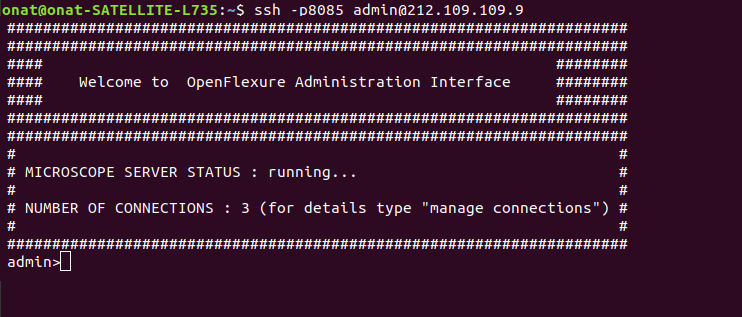
\includegraphics[scale=0.5]{Figures/admin_interface}
			\caption{OpenFlexure Administration Command-line Interface}
			\label{fig:system_admin_management_interface}
		\end{figure}
		\item \textbf{Maintainer Command-line Interface} \\
		Similar to system administrators, maintainers use a separate maintainer command-line interface to do their tasks, due to the similar reasons. Since the permissions of the maintainers are limited to viewing released updates, updating the system and retrieving the system logs, commands available to maintainers are also limited. Maintainers can list saved error logs, system details such as the current software version and the information about the latest software updates. Furthermore, maintainers are also able to update the system software using the command provided by this interface. Maintainer command-line interface is provided by a bash script placed inside the local microscope server and starts to run when a maintainer connects to the microscope using SSH.
	\end{itemize}
	\textbf{Design Rationale:} 
	\begin{enumerate}
		\item The reason to use a command-line interface rather than GUI is related to speed. Maintainers should be able to apply their actions immediately. Since the command-line interface is a more quick way to apply actions, it is preferred over GUI.
	\end{enumerate}
	\paragraph{System/Service Interfaces}
	\paragraph{Interface between Web API and Gallery}
	The interface provided by the Gallery is used by the Web API when a user sends a request to the Web API to display/edit/manage the saved media materials.
	\subparagraph{Design Rationale:}
	\begin{itemize}
		\item User sends a request to the Web API to view/edit the stored media.
		\item To allow the Web API to use the media facilities that user wants to use, Gallery provides this interface and based on the request sent to the Web API, corresponding operation of the Gallery is activated.
		\item This interface is related to the Open Gallery and Modify Media functions defined in the use-case diagram.
	\end{itemize}
	\paragraph{Interface between Web API and Position Controller}
	The interface provided by the Position Controller is used by the Web API when a user sends a request to the Web API to move the position of the stage.
	\subparagraph{Design Rationale:}
	\begin{itemize}
		\item User sends a request to the Web API to navigate the positions of the microscope stage.
		\item To allow the Web API to change the position of the stage to the desired position, Position Controller provides this interface and changes the positions of the stage using the provided coordinates.
		\item This interface is related to the Navigate Stage function defined in the use-case diagram.
	\end{itemize}
	\paragraph{Interface provided Web API and Display Controller}
	The interface provided by the Display Controller is used by the Web API when a user sends a request to display the livestream, capture the current view, record to the livestream or scan an area.
	\subparagraph{Design Rationale:}
	\begin{itemize}
		\item User sends a request to the Web API to use facilities provided by the Display Controller such as viewing livestream, capturing images, recording videos etc.
		\item To allow the Web API to use the mentioned facilities that user wants to use, Display Controller provides this interface and based on the request sent to the Web API, corresponding operation of the Display Controller is activated.
		\item This interface is related to the View Livestream, Capture Image, Record Video and Scan functions defined in the use-case diagram.
	\end{itemize}

\subsubsection{Sequence Diagrams}
\begin{figure}[H]
	\centering
	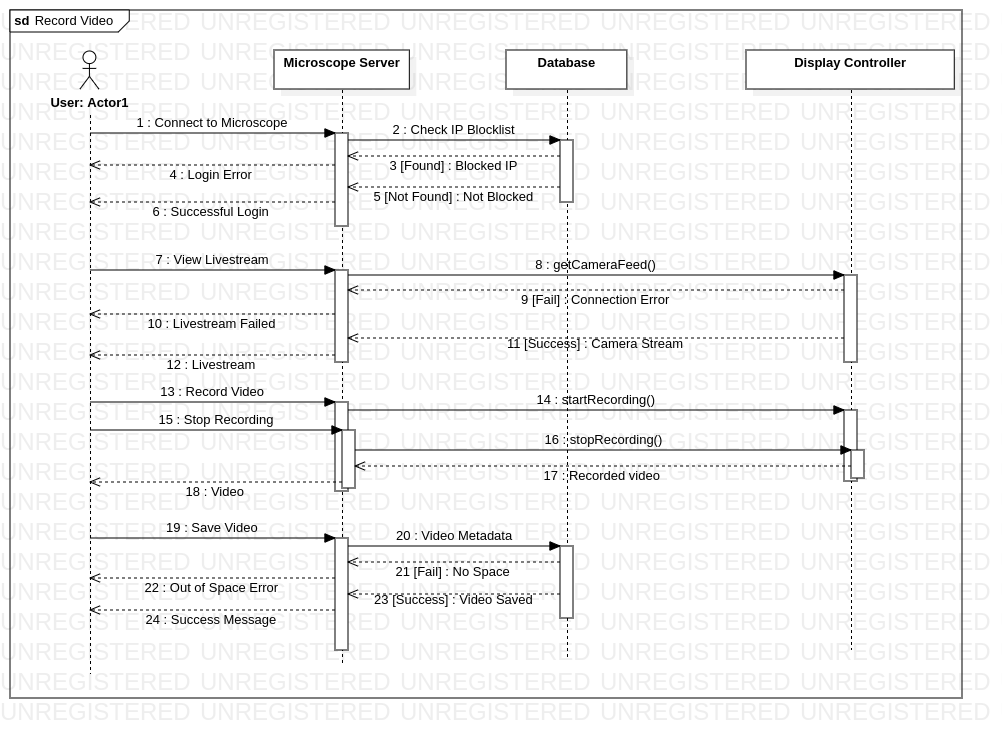
\includegraphics[scale=0.4]{Uml_Images/record_video_seq_diagram}
	\caption{Sequence Diagram of Record Video Function}
	\label{fig:record_video_seq_diagram}
\end{figure}
\begin{figure}[H]
	\centering
	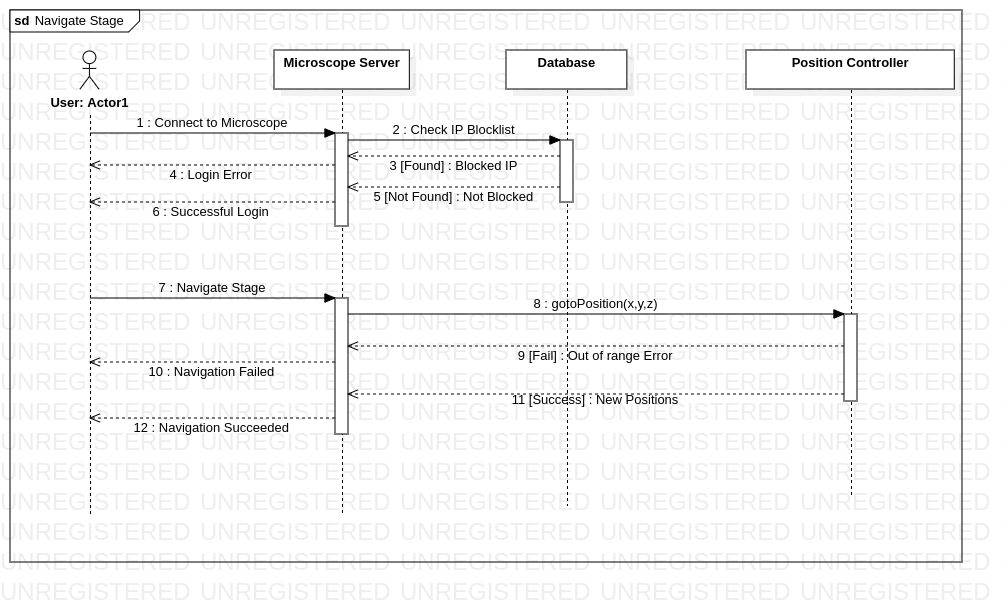
\includegraphics[scale=0.4]{Uml_Images/navigate_stage_seq_diagram}
	\caption{Sequence Diagram of Navigate Stage Function}
	\label{fig:navigate_stage_seq_diagram}
\end{figure}
\begin{figure}[H]
	\centering
	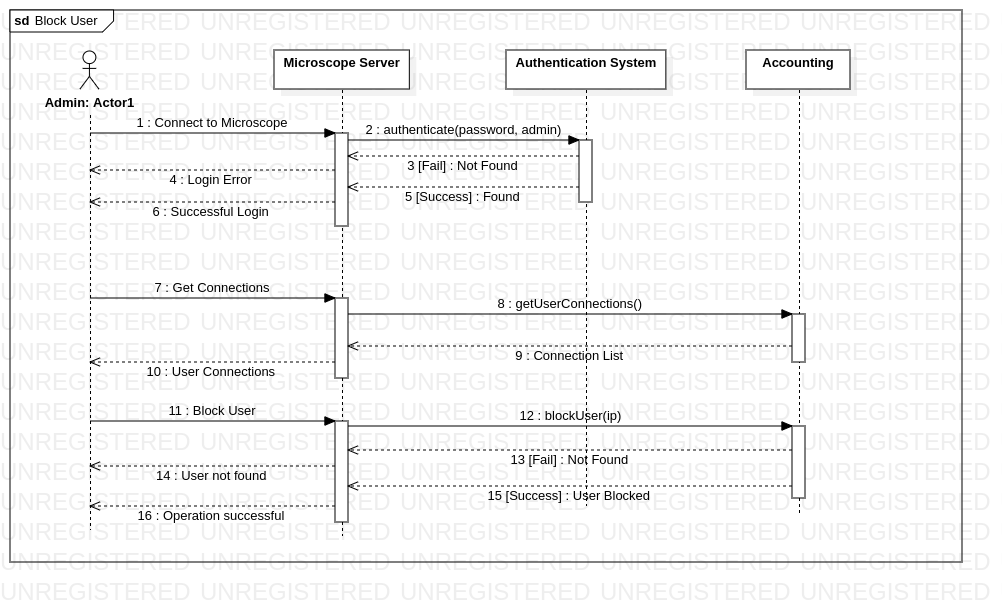
\includegraphics[scale=0.4]{Uml_Images/block_user_seq_diagram}
	\caption{Sequence Diagram of Block User Function}
	\label{fig:block_user_seq_diagram}
\end{figure}
\begin{figure}[H]
	\centering
	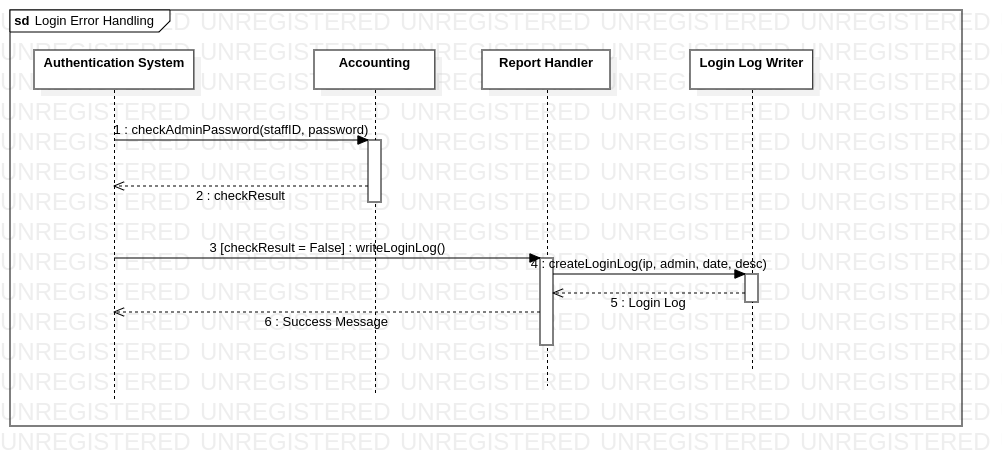
\includegraphics[scale=0.4]{Uml_Images/login_error_seq_diagram}
	\caption{Sequence Diagram of Login Error Handling}
	\label{fig:login_error_handling_seq_diagram}
\end{figure}
\begin{figure}[H]
	\centering
	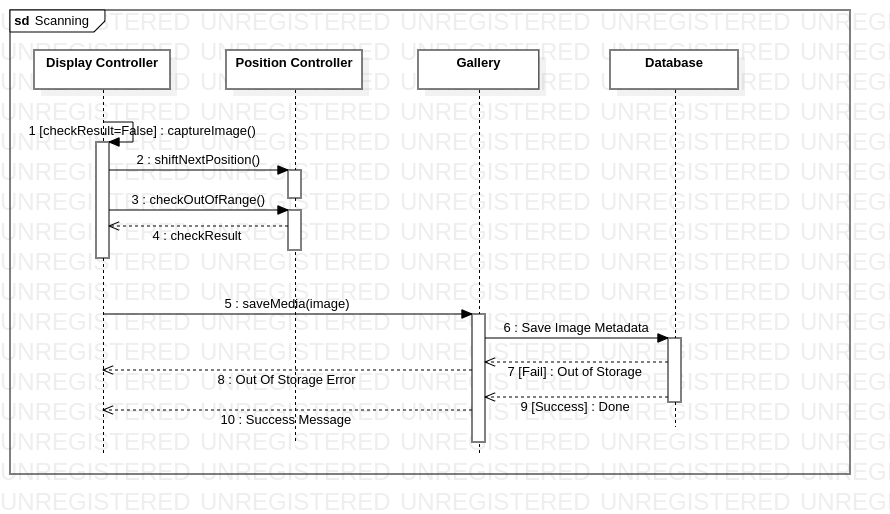
\includegraphics[scale=0.4]{Uml_Images/scanning_seq_diagram}
	\caption{Sequence Diagram of Scanning}
	\label{fig:scanning_seq_diagram}
\end{figure}
\subsubsection{Design Rationale}
Design rationales are specified where each interface is defined above.